% ============================================================================
\section{Parallel, flow, and diffusion acoustic models}
% ============================================================================

\begin{frame}{FastSpeech 2: parallel mel generation}
  \begin{itemize}\footnotesize
    \item FastSpeech~2 uses a Feed-Forward Transformer with a Length Regulator to match phoneme and spectrogram lengths, replacing soft attention.
    \item The Variance Adaptor predicts duration, pitch, and energy for more control over prosody.
    \item Together they address the ``one-to-many'' mapping: the Duration Predictor decides exactly how many frames each phoneme lasts, which also makes the system more stable.
    \item Pitch Predictor models the fundamental frequency ($F_0$); Energy Predictor models the loudness (from the spectrogram).
  \end{itemize}
  \centering
  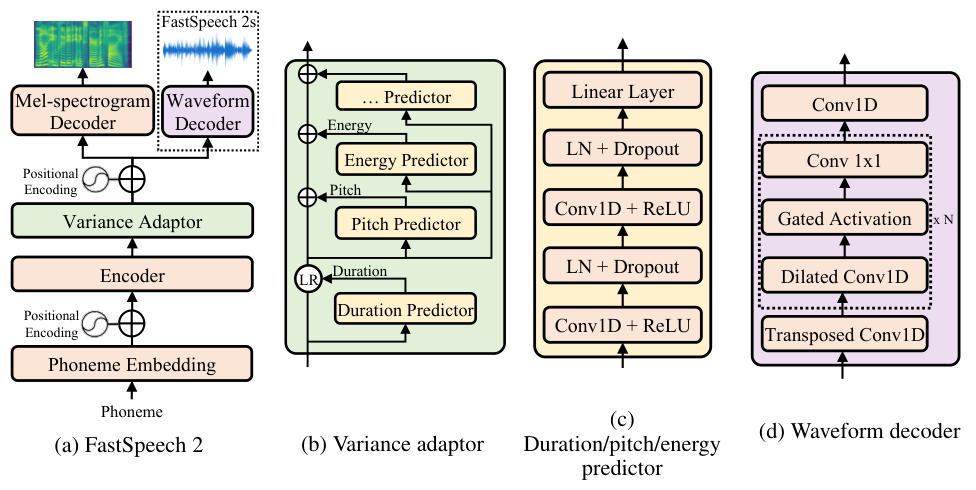
\includegraphics[width=0.92\textwidth,height=0.46\textheight,keepaspectratio]{images/tts/fastspeech2_architecture_paper.png}
  \slideimgsource{Ren et al., ``FastSpeech 2: Fast and High-Quality End-to-End Text to Speech,'' Fig.~1; \href{https://arxiv.org/abs/2006.04558}{arXiv:2006.04558}.}
\end{frame}

\begin{frame}{From noise to speech: flows, diffusion, and flow matching}
  \begin{itemize}\footnotesize\itemsep0.35em
    \item Once durations are predicted, the acoustic model only has to turn a noise sample into speech features. Three families do that, and they differ mainly in how many network passes one utterance costs.
    \item \textbf{Normalizing flow:} an invertible network maps speech features to a simple Gaussian. Training maximizes exact likelihood; generating runs the same network backwards on a noise sample, in a single pass. Used by Glow-TTS and inside VITS.
    \item \textbf{Diffusion:} a fixed forward process adds noise to the features until nothing is left but noise; the model learns to undo one step of it, so generating means denoising repeatedly, tens to hundreds of passes. Used by Grad-TTS.
    \item \textbf{Flow matching:} rather than a noising process, the model regresses the \emph{velocity} along a straight path from noise to data. Generating integrates that velocity field with an ODE solver, which needs far fewer steps than diffusion for comparable quality. Used by Voicebox and F5-TTS.
    \item All three are conditioned on the text, so choosing between them is mostly a quality-versus-latency decision.
  \end{itemize}
\end{frame}

\begin{frame}{Glow-TTS and monotonic alignment search (MAS)}
  \begin{itemize}\footnotesize
    \item Glow-TTS uses Normalizing Flows to turn a simple distribution into a mel-spectrogram distribution.
    \item Monotonic Alignment Search (MAS) finds the single best monotonic path between text and speech using dynamic programming.
    \item Unlike soft attention, MAS avoids alignment breaks, so the model works well on long utterances.
  \end{itemize}
  \centering
  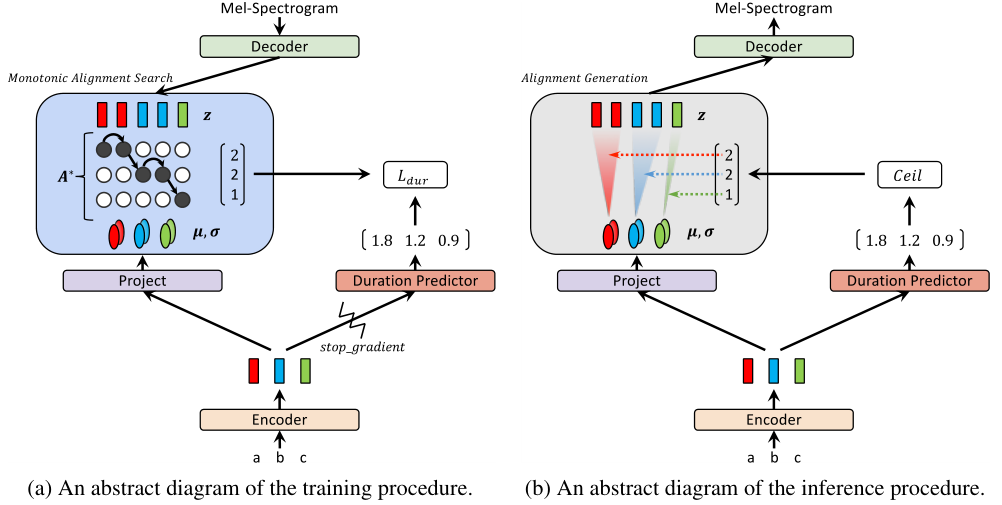
\includegraphics[width=0.90\textwidth,height=0.40\textheight,keepaspectratio]{images/tts/glowtts_training_inference.png}
  \slideimgsource{Kim et al., ``Glow-TTS: A Generative Flow for Text-to-Speech via Monotonic Alignment Search,'' Fig.~1; \href{https://arxiv.org/abs/2005.11129}{arXiv:2005.11129}.}
\end{frame}

\begin{frame}{Grad-TTS: diffusion in the acoustic domain}
  \begin{itemize}\footnotesize
    \item Grad-TTS uses score-based diffusion to turn random noise into structured mel-spectrograms.
    \item The reverse diffusion process is controlled by stochastic differential equations (SDEs).
    \item Users can control the trade-off between quality and speed by choosing the number of reverse steps.
    \item Grad-TTS can sound good with as few as 10 steps, and it is faster and more robust than Tacotron~2.
  \end{itemize}
  \centering
  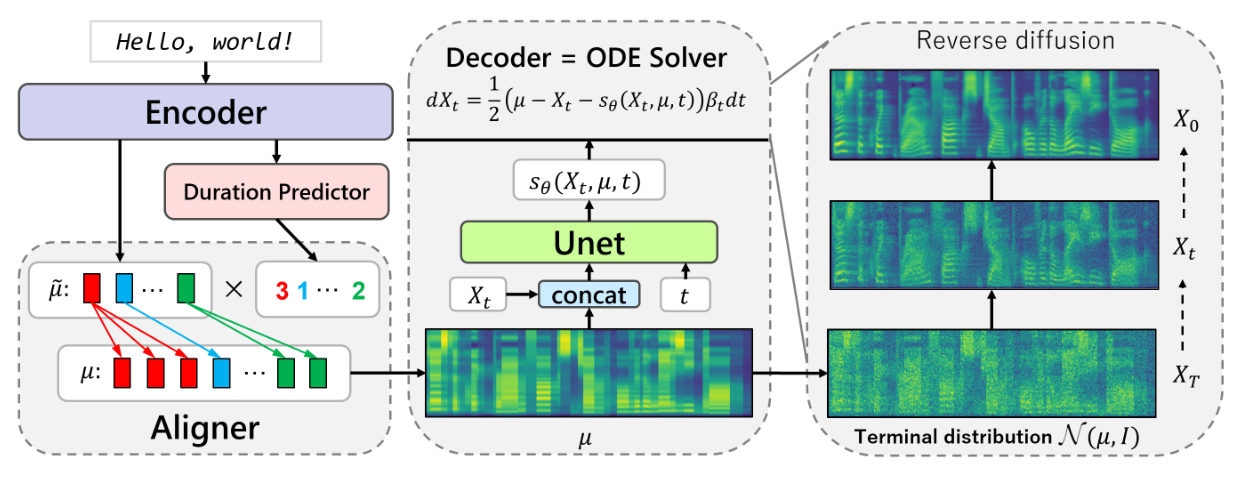
\includegraphics[width=0.95\textwidth,height=0.38\textheight,keepaspectratio]{images/tts/gradtts_fig2_inference.png}
  \slideimgsource{Popov et al., ``Grad-TTS: A Diffusion Probabilistic Model for Text-to-Speech,'' Fig.~2; \href{https://arxiv.org/abs/2105.06337}{arXiv:2105.06337}.}
\end{frame}

\begin{frame}{HiFi-GAN and parallel front ends}
  \begin{itemize}\footnotesize
    \item HiFi-GAN is a vocoder trained as a \textbf{generative adversarial network} (GAN): the generator turns mel-spectrograms into a waveform, discriminators try to tell its output from real recordings, and the generator improves by fooling them.
    \item The generator upsamples mel frames to waveform resolution with transposed convolutions; each stage passes through a multi-receptive field fusion (MRF) module that sums residual blocks with different kernel sizes and dilation rates, so short and long patterns are modelled together.
    \item Pairing it with a parallel front end like FastSpeech, which produces all mel frames at once, gives a fast and high-quality stack.
  \end{itemize}
  \centering
  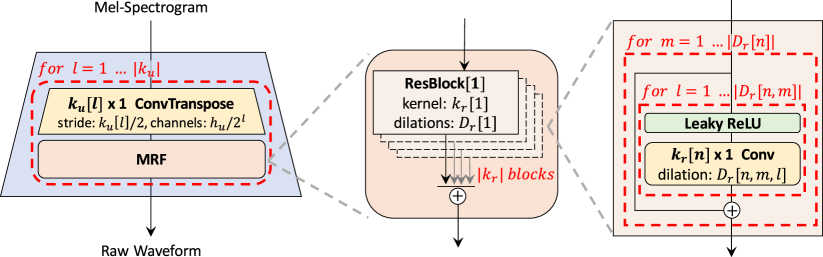
\includegraphics[width=0.95\textwidth,height=0.40\textheight,keepaspectratio]{images/tts/hifigan_generator_mrf_fig1.png}
  \slideimgsource{Kong et al., ``HiFi-GAN: Generative Adversarial Networks for Efficient and High Fidelity Speech Synthesis,'' Fig.~1; \href{https://arxiv.org/abs/2010.05646}{arXiv:2010.05646}.}
\end{frame}

\begin{frame}{VITS: variational inference for end-to-end TTS}
  \begin{itemize}\footnotesize
    \item Trains as a conditional \textbf{variational autoencoder} (VAE): a posterior encoder maps real mel frames to a distribution over latent features and the waveform decoder reconstructs audio from a sample of it, so acoustic model and vocoder become one network.
    \item At training: monotonic alignment search (MAS) links text to speech, and a discriminator on the generated waveform supplies the adversarial loss.
    \item At inference: text $\rightarrow$ text encoder + duration predictor $\rightarrow$ latent features $\rightarrow$ waveform decoder $\rightarrow$ audio (no separate vocoder).
  \end{itemize}
  \centering
  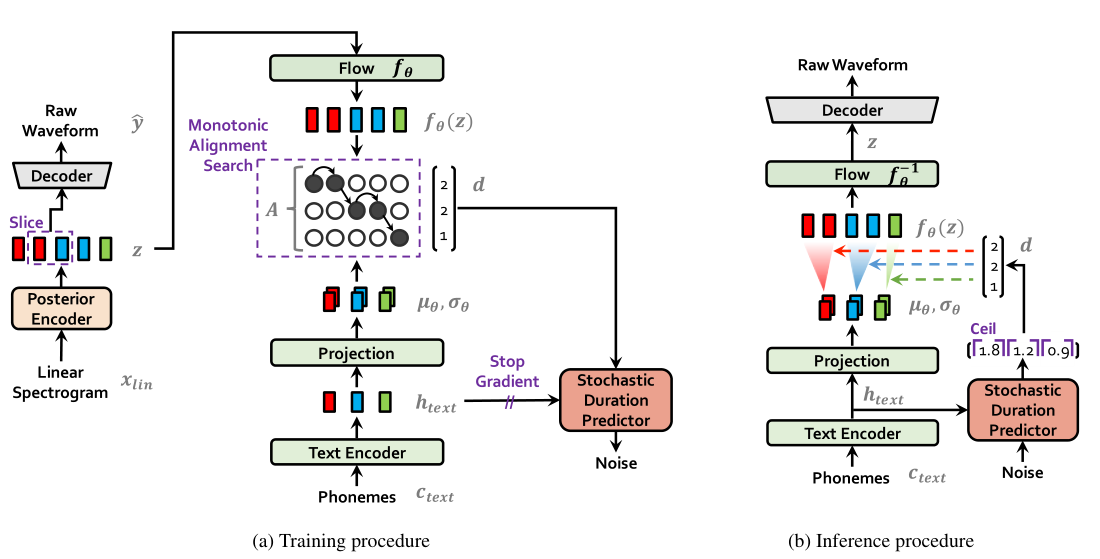
\includegraphics[width=0.98\textwidth,height=0.40\textheight,keepaspectratio]{images/tts/vits_fig1_architecture.png}
  \slideimgsource{Kim, Kong, and Son, ``Conditional Variational Autoencoder with Adversarial Learning for End-to-End Text-to-Speech'' (VITS), Fig.~1; \href{https://arxiv.org/abs/2106.06103}{arXiv:2106.06103}.}
\end{frame}
